\chapter{Input-Output approach}
We will work either with static and dynamical systems of the following forms, note that can exist also systems dependent on partial derivative but we will not see them.

\[
\begin{aligned}
&S_{\text{static}}: y(t)=g(u(t))\\
&S_{\text{dynamical}}: \begin{cases}
	\dot{x}(t)=f(x(t),u(t)), \quad x(0)=x_0\\
	y(t)=g(x(t),u(t))
\end{cases}
\end{aligned}
\]
The input-output approach for system analysis and design take a different perspective and looks at the systems as an operator that maps input signal into output signals.
\begin{figure}[H]
	\centering
	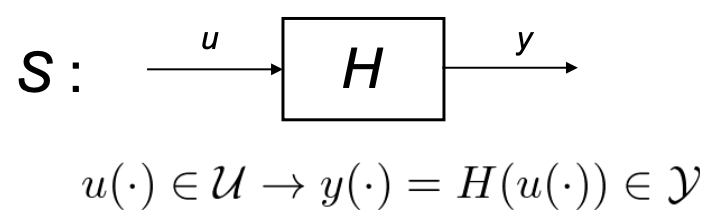
\includegraphics[scale=0.4]{immagini/IOsys}
	\caption{$H:\mathcal{U}\to \mathcal{Y}$ Input-output operator (I/O)}
	\label{fig:iosys}
\end{figure}
Note that if S is a dynamical system, the initial state $x_0$ must be fixed. As $x_0$ varies, S defines a family of I/O operators. What we need to describe the system, either static or dynamic, uniformly as an operator is a notion of input and output function spaces, so a space where the input and output signals take place.
\subsubsection{Input and Output function spaces}
 For what concern control we are interested in signals which are, looking at SISO system for simplicity, represented by a function defined from $\Re^+$ taking values in $\Re$ which can be continuous time or piecewise continuous (such as a step). \[v(\cdot):\Re^+\to\Re\] where $v(\cdot)\in\mathcal{V}$ and 
$\mathcal{V}$ is a normed linear space. Let's define what is a \emph{normed linear space}.
\[
\left.
\begin{aligned}
	&v_1(\cdot)+v_2(\cdot)\in\mathcal{V},\,\forall\,v_1(\cdot),\,v_2(\cdot)\in\mathcal{V}\\
	&\alpha v(\cdot)\in\mathcal{V},\,\forall v(\cdot)\in\mathcal{V},\alpha\in \Re
\end{aligned}
\right\rbrace \text{linear}
\]
\[
\left.
\begin{aligned}
	&\text{equipped with a function} \, \|\cdot\|:\mathcal{V}\to\Re^+\text{that satisfies}\\
	&1) \|v(\cdot)\| = 0 \Rightarrow v(\cdot)\equiv 0\\
	&2)\|\alpha v(\cdot)\|=|\alpha|\|v(\cdot)\|,\forall\,\alpha\in\Re,\,\forall\, v(\cdot)\in\mathcal{V}\\
	&3)\|v_1(\cdot)+v_2(\cdot)\|\le\|v_1(\cdot)\|+\|v_2(\cdot)\|,\,\forall\, v_1(\cdot),v_2(\cdot)\in\mathcal{V}
\end{aligned}
\right\rbrace\text{normed}
\]
\paragraph{Lebesgue space}
We are not interested in general linear normed spaces but we will extend them starting from Lebesgue space.
\[
\begin{aligned}
	&L_p:=\{v(\cdot):\Re^+\to\Re:\quad \|v(\cdot\|_p<\infty)\}\\
	&\text{where} \|v(\cdot)\|_p:=\begin{cases}
	\left(	int_{0}^{\infty}|v(t)|^pdt\right)^{\frac{1}{p}},& 0<p<\infty\\
	\sup_{t\in\Re^+}|v(t)|&p=\infty
	\end{cases}
\end{aligned}
\]
\begin{itemize}
	\item $p=1 \to$ absolutely integrable signal
	\item $p=2 \to$ finite energy signal
	\item $p=\infty	\to$  uniformly bounded signal
\end{itemize}
\begin{note}
	we shall use the symbol $\mathcal{L}$ to denote a generic $L_p$ space.
\end{note}




%%examples can added%%%%




In general, a system fed by an $L_p$ input signal does not provide an output signal in $L_p$ (e.g., a dynamical system that is unstable), that leds us to \textcolor{red}{extended Lebesgue spaces}.
\paragraph{Extended Lebesgue space}
\[
\begin{aligned}
	&\mathcal{L}_e:=\{v(\cdot):\Re^+\to\Re:\quad v_{\tau}(\cdot) \in \mathcal{L},\forall\,\tau \in\Re^+\}\\
	&\text{where} v_{\tau}(\cdot) \text{is the truncation of} v(\cdot) \text{at time} \tau
	&\begin{cases}
		v(t), & t\in[o,\tau]\\
		0, & t>\tau
	\end{cases}
\end{aligned}
\]
\begin{figure}[H]
	\centering
	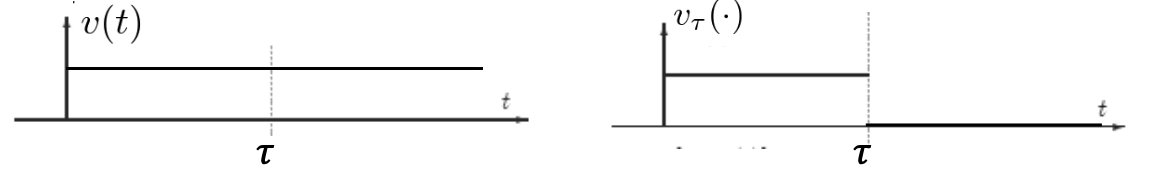
\includegraphics[scale=0.4]{immagini/elebtruncation}
	\caption{}
	\label{fig:elebtruncation}
\end{figure}
We apply this truncation because in this way we can compute a finite integral
\begin{remark}
	\begin{itemize}
		\item This includes signals that grow unbounded as t, $e^t$, $e^tsen(t)$, and, allows to describe dynamical systems with unbounded output
		\item $v(\cdot)\in \mathcal{L}$ if and only if $\exists M: \|v_{\tau}(\cdot)\|<M,\forall\,\tau\ge0$
		\item $\mathcal{L}\in\mathcal{L}_e$
	\end{itemize}
\end{remark}
In control we are interest only in \textcolor{red}{causal systems (operators)} because we have to use signal in real time.
\paragraph{Causal operator}
\begin{defn}
		System S (operator H) from $\mathcal{L}_e$ to $\mathcal{L}$ is causal if \[H(u(\cdot))_{\tau}=H(u(\cdot)_{\tau})_{\tau}\qquad \forall\, u(\cdot)\in\mathcal{L}_e,\, \forall\, \tau \in \Re^+\]
that is the Behavior of y up to time $t=\tau$ is independent of the behavior of u for $t>\tau$, for every signal $u(\cdot)$ and for every $\tau$
\end{defn}
\begin{figure}[H]
	\centering
	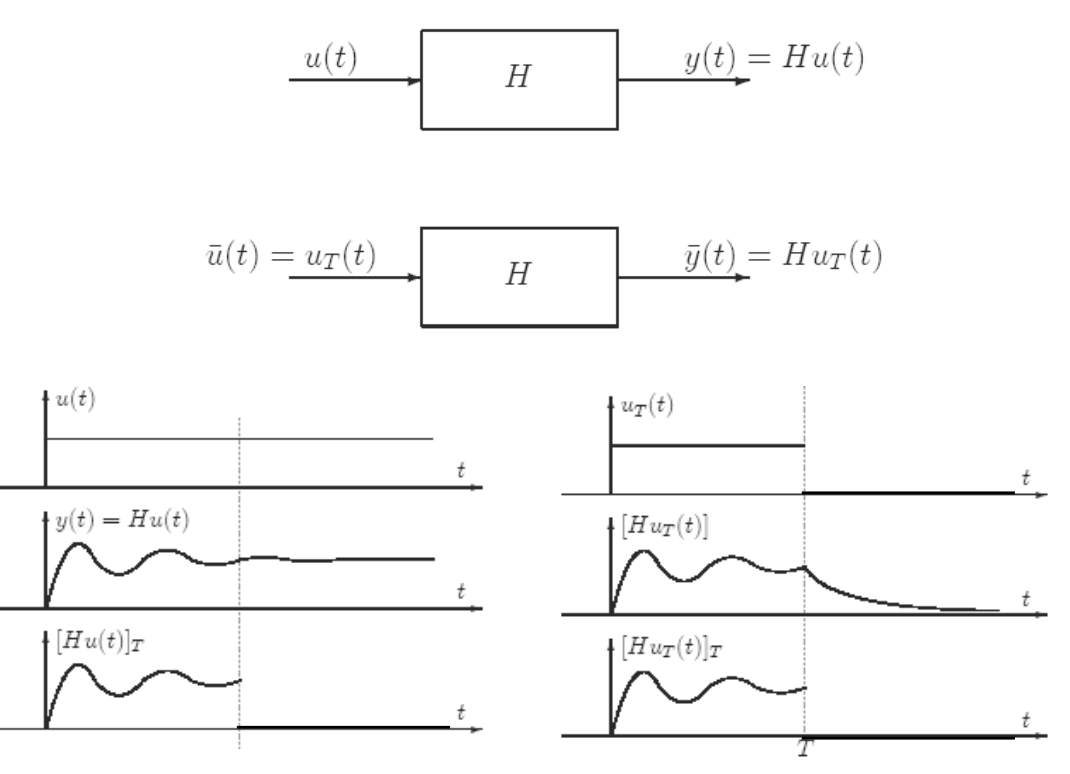
\includegraphics[scale=0.4]{immagini/causal}
	\caption{}
	\label{fig:causal}
\end{figure}
\paragraph{Weakly bounded operator}
Our aim is to be able to describe the Behavior of the system and formalize  the notion of stability in this set-up, but before we need some notions and definitions.
\begin{defn}[weakly bounded operator]
	A causal operator $H:\mathcal{L}_e\to\mathcal{L}_e$ is weakly bounded (or with finite gain) if \[
	\exists \hat{\gamma},\hat{\beta}\in\Re^+:\quad \|H(u(\cdot))\|\le\hat{\gamma}\|u(\cdot)\|+\hat{\beta},\,\forall\, u(\cdot)\in \mathcal{L}
	\]
\end{defn}
\begin{defn}
	Let $H:\mathcal{L}_e\to\mathcal{L}_e$ be a causal weakly bounded operator. The gain of H is given by
	\[\gamma(H):=\inf\{\hat{\gamma}\in\Re^+|\exists\hat{\beta}\in\Re^+:\quad\|H(u\cdot)\|\le\hat{\gamma}\|u(\cdot)\|+\hat{\beta},\forall \, u(\cdot)\in \mathcal{L}\}\]
\end{defn}
\begin{defn}[biased operator]
	The operator H from $\mathcal{L}_e$ to $\mathcal{L}_e$ is biased if
	\[
	\begin{aligned}
		H(0)=&y_0(\cdot)\neq0\\
		&u(\cdot)\equiv0
	\end{aligned}
	\]
\end{defn}
If H is biased then we can define the \textbf{unbiased operator G associated with H:}\[
G:\mathcal{L}_e\to\mathcal{L}_e\quad u(\cdot)\in\mathcal{L}\to G(u(\cdot))=H(u(\cdot))-yo(\cdot)\in \mathcal{L}_e
\]
\begin{figure}[H]
	\centering
	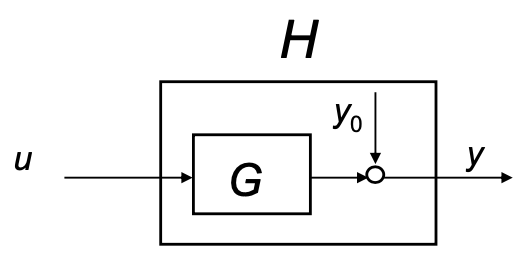
\includegraphics[scale=0.4]{immagini/biaed}
	\caption{}
	\label{fig:biaed}
\end{figure}
\paragraph{Example: linear asymptotically stable dynamical system}
\[
\begin{aligned}
	&\begin{cases}
		\dot{x}=Ax+Bu, &x(0)=x_0 \in \Re^n\\
		y=Cx
	\end{cases}
&Re[\lambda_i(A)]<0,\quad i=1,2,\dots,n\\
&y(t)=Ce^{At}x_0+\int_{0}^{t}Ce^{A(t-\tau)}Bu(\tau)d\tau,t\in\Re^+,\, \forall u(\cdot)\in\mathcal{L}_e\\
&g(t)=Ce^{At}B,\, t\in\Re^+ \text{impulse response of S} (g(t)=0, t<0)\\
&y(t)=Ce^{At}x_0+\int_{0}^{t}g(t-\tau)u(\tau)d\tau, t \in\Re^+, \, u(\cdot)\in \mathcal{L}_e\\
&S:\quad y(\cdot)=H(u(\cdot))=G(u(\cdot))+y_0(\cdot)\in\mathcal{L}_e,\quad \forall u(\cdot) \in \mathcal{L}_e
&y_0(t)=Ce^{At}x_0, t\in \Re^+\\
&G(u(\cdot)):=\int_{0}^{t}g(t-\tau)u(\tau)d\tau=g(\cdot)*u(\cdot)	
\end{aligned}
\] The operator H is causal and biased if $y_0(\cdot)\equiv 0$. Let $\boxed{\mathcal{L}=L_{\infty}}$, is H weakly bounded?\[
\begin{aligned}
	&y_0(t)=Ce^{At}x_0, t \in \Re^+ \quad \text{free evolution of S}\\
	&\sup_{t\in\Re^+} |y_0(t)|<\infty \to y_0(\cdot) \in L_{\infty} \to \beta := \|y_0(\cdot)\|_{infty}\\
	&\|G\|:=\sup_{u\in\mathcal{L}\smallsetminus\{0\}}\frac{\|Gu(\cdot)\|}{\|u(\cdot\|)}\quad \text{induced norm of G}\\
	&\text{if the induced norm is finite then} 	\, \|G(u(\cdot))\|\le\|G\|\|u(\cdot)\|,\forall u \in \mathcal{L}\\
	&\|G\|:=\sup_{u\in\mathcal{L}\smallsetminus\{0\}}\frac{\|Gu(\cdot)\|}{\|u(\cdot\|)}=\sup_{\|u(\cdot)\|=1}\frac{\|Gu(\cdot)\|}{\|u(\cdot\|)}\\
	&\|G\|_{\infty}=\sup_{\|u(\cdot)\|_{\infty}=1}\|G(u(\cdot))\|_{\infty}=\sup_{\|u(\cdot)\|_{\infty}=1}\sup_{t\ge0} \left | \int_{0}^{t}g(t-\tau)u(\tau)d\tau \right |\\
	&\le\sup_{\|u(\cdot)\|_{\infty}=1}\sup_{t\ge0}\int_{0}^{t}|g(t-\tau)||u(\tau)|d\tau\le\sup_{t\ge0}\int_{0}^{t}|g(t-\tau)|d\tau \\
	&\|G\|_{\infty} \le\sup_{t\ge0}\int_{0}^{t}|g(t-\tau)|d\tau = \sup_{t\ge0}\int_{0}^{t}|g(\tau)|d\tau=\int_{0}^{\infty}|g(\tau)d\tau \\
	&\text{where} 	\, g(t)=Ce^{At}B, \, t\in \Re^+ \text{impulse response of S}\\
	&\int_{0}^{\infty}|g(t)|dt<\infty\to g(\cdot)\in L_1 \to k_1 := \|g(\cdot)\|_1\\
	&\text{H is weakly bounded because:}\\
	&\|y(\cdot)\|_{\infty}=\|G(u(\cdot))+y_0(\cdot)\|_{\infty}\le\|G(u(\cdot))\|_{\infty}+\|y_0(\cdot)\|_{\infty}\\
	&\le k_1\|u(\cdot)\|_{\infty}+\beta,\, \forall u(\cdot) \in L_{\infty}\\
	&\text{and the gain, following the definition before}\\
	&\gamma_{\infty}(H)\ge k_1\\
	&\text{One can show that} \, \gamma_{\infty}(H)=k_1\\
\end{aligned}
\]Let, now $\boxed{\mathcal{L}=L_2}$ one can show that H is weakly bounded with gain \[\gamma_2(H)=\max_{\omega\in\Re^+}|F(j\omega)|\] The H operator is weakly bounded, with gain equal to the induced norm of G in $L_{pe}$, for any p.
\section{Input-Output stability}
\begin{defn}[$\mathcal{L}$ stability]
	A causal operator $H:\mathcal{L}_e\to\mathcal{L}_e$ is $\mathcal{L}$-stable if $H(\mathcal{L})\subseteq\mathcal{L}$, that is $H(u(\cdot))\in\mathcal{L},\quad \forall \, u(\cdot)\in\mathcal{L}$
	\begin{itemize}
		\item If $\mathcal{L}=L_{\infty}\to$ BIBO(bounded input bounded output) stability
		\item It is a property of the system
		\item It applies to both static and dybamic systems
		\item It depends on $\mathcal{L}$
	\end{itemize}
\end{defn}
\begin{thm}[Weakly boundedness implies $\mathcal{L}$-stability]
	A causal weakly bounded operator $H:\mathcal{L}_e\to\mathcal{L}_e$ is $\mathcal{L}$-stable since 
	\[
	\exists \hat{\gamma},\hat{\beta}\in\Re^+:\|H(u(\cdot))\|\le\hat{\gamma}\|u(\cdot)\|+\hat{\beta},\forall u(\cdot)\in\mathcal{L}
	\]where $\hat{\gamma}$ is the finite gain of the $\mathcal{L}$-stability
\end{thm}
\subsection{Stability of interconnected systems}
\subsubsection{Cascade}
\begin{figure}[H]
	\centering
	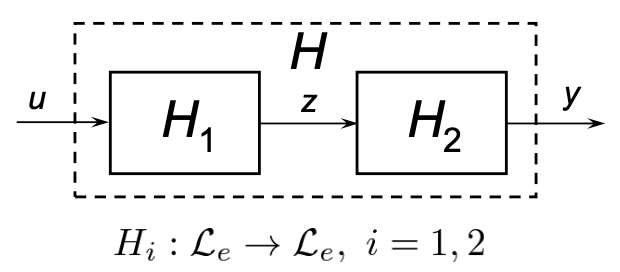
\includegraphics[scale=0.4]{immagini/cascio}
	\caption{}
	\label{fig:cascio}
\end{figure}
\begin{thm}
	Two causal and weakly bounded operators $H_1$ and $H_2$, interconnected in cascade, originates an operators $H$ 
	\[
	u(\cdot)\in\mathcal{L}_e\to y(\cdot)=H(u(\cdot))=H_2(H_1(u(\cdot)))\in\mathcal{L}_e
	\] 
	causal and weakly bounded with gain $\gamma(H)\le\gamma(H_1)\gamma(H_2)$
\end{thm}
\begin{proof}
	$H_1$ weakly bounded implies that
	\[\exists \gamma_1,\beta_1\in\Re^+:\|H_1(u(\cdot))\|\le\gamma_1\|u(\cdot)\|+\beta_1,\forall\, u(\cdot)\in\mathcal{L}\to z(\cdot)=H_1(u(\cdot))\in\mathcal{L}    \]
	
	$H_2$ weakly bounded implies that
	\[\exists \gamma_2,\beta_2\in\Re^+:\|H_2(z(\cdot))\|\le\gamma_2\|z(\cdot)\|+\beta_2,\forall z(\cdot)\in\mathcal{L}  \]
	Then
	\[
	\|H(u(\cdot))\|=\|H_2(H_1(u(\cdot)))\|\le\gamma_2(\gamma_1\|u(\cdot)\|+\beta_1)+\beta_2=\gamma_2\gamma_1\|u(\cdot)\|+\gamma_2\beta_1+\beta_2,\forall u(\cdot)\in\mathcal{L}
	\]
	that is H is weakly bounded and $\gamma(H)\le\gamma(H_1)\gamma(H_2)$
\end{proof}

\subsubsection{Parallel}
\begin{figure}[H]
	\centering
	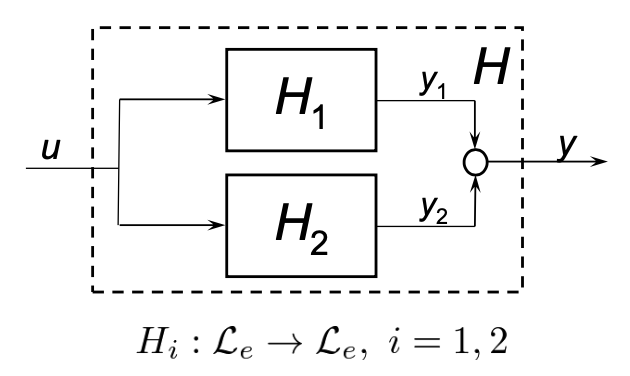
\includegraphics[scale=0.4]{immagini/parallelio}
	\caption{}
	\label{fig:parallelio}
\end{figure}
\begin{thm}
	Two causal and weakly bounded operators $H_1$ and $H_2$, interconnected in parallel, originates an operator $H$  \[u(\cdot)\in\mathcal{L}_e\to y(\cdot)=H_1(u(\cdot))+H_2(u(\cdot))\in \mathcal{L}_e\] causal and weakly bounded with gain $\gamma(H)\le\gamma(H_1)+\gamma(H_2)$
\end{thm}
\subsubsection{Feedback}
\begin{figure}[H]
	\centering
	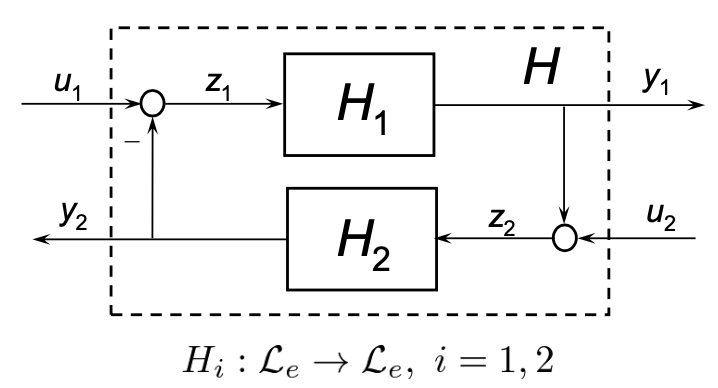
\includegraphics[scale=0.4]{immagini/feedbackio}
	\caption{}
	\label{fig:feedbackio}
\end{figure}
\begin{itemize}
	\item The operator H has two inputs and two outputs. Let us define the operators with one input and one output:
	\[
	H_{ij}:\mathcal{L}_e\to\mathcal{L}_e \qquad y_i(\cdot)=H_{ij}(u_j(\cdot)),i,j=1,2
	\]
	\item The operator H is well-posed if the pair $(y_1,y_2) $ exists and is unique for any $(u_1,u_2)\in \mathcal{L}_e\times\mathcal{L}_e$
\end{itemize}
\paragraph{Small gain theorem}
\begin{thm}[Small gain theorem]
	Let H be a well-posed causal operator obtained by connecting in feedback two causal and weakly bounded operators $H_1$ and $H_2$. If \[\lambda:=\gamma(H_1)\gamma(H_2)<1\] then, H is weakly bounded, that is: \[
	\exists \hat{\gamma}_{i1},\hat{\gamma}_{i2},\hat{\beta}_i \, \in\,\Re^+:\, \|y_i(\cdot)\| \le \hat{\gamma}_{i1}\| u_1(\cdot)  \|+\hat{\gamma}_{i2}\|u_2(\cdot)\|+\hat{\beta}_i\quad 	\forall \, u_1(\cdot),u_2(\cdot)\in\mathcal{L},\, i=1,2	
	\]
	Furthermore,
	\[
	\gamma(H_{11})\le \frac{\gamma(H_1)}{1-\lambda},\,\gamma(H_{22})\le \frac{\gamma(H_2)}{1-\lambda},\, \gamma(H_{12}),\,\gamma(H_{21})\le\frac{\lambda}{1-\lambda}
	\]
\end{thm}
\subsubsection{Example: Lur'e system with input}
\begin{figure}[H]
	\centering
	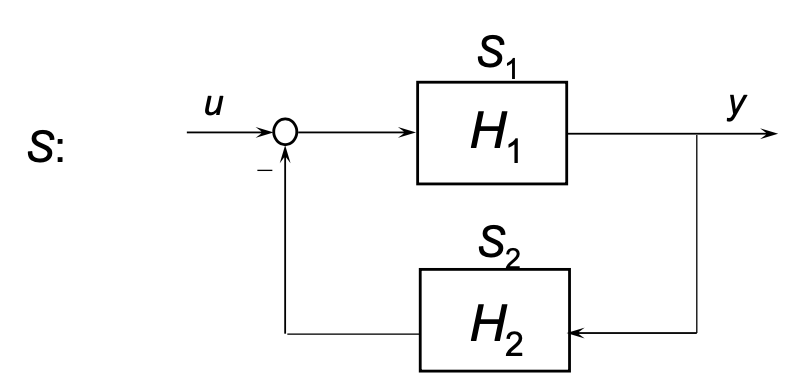
\includegraphics[scale=0.4]{immagini/lureinput}
	\caption{}
	\label{fig:lureinput}
\end{figure}
$S_1$ is a linear time invariant dynamical system that is asymptotically stable and strictly proper with transfer function G(s) $\to$ causal and weakly bounded in $L_p$. For this reason:\[
\gamma(H_1)=\begin{cases}
	\max_{\omega\ge0}|G(j\omega)|:=G_{max}, &\mathcal{L}=L_2\\
	\int_{0}^{\infty}|g(t)|dt:=k_1, & \mathcal{L}=L_{\infty}
\end{cases}
\]
While $S_2$ is static system with sector non linearity $\phi(\cdot)$ in $[-k,\, k]$ and $|\phi(v)|\le k|v|.\,\forall\, v \in\Re$
\begin{itemize}
	\item $\mathcal{L}=L_{\infty}\to \gamma(H_2)\le k$ \\because $\|H_2(u(\cdot))\|_{\infty}=\sup_{t\ge0}|\phi(u(t))|\le k \sup_{t\ge0}|u(t)|\le k \|u\|_{\infty},\forall u \in L_{\infty}$
	\item $\mathcal{L}=L_{2}\to \gamma(H_2)\le k$ \\because\[
	\|H_2(u(\cdot))\|_2^2=\int_{0}^{\infty}\phi^2(u(t))ft \le \int_{0}^{\infty}k^2u^2(t)dt=k^2\|u(\cdot)\|^2_2,\quad\forall\, u(\cdot) \in\L_2
	\]
\end{itemize}
\section{$L_2$ stability in sector $[k_1,k_2]$}
\begin{figure}[H]
	\centering
	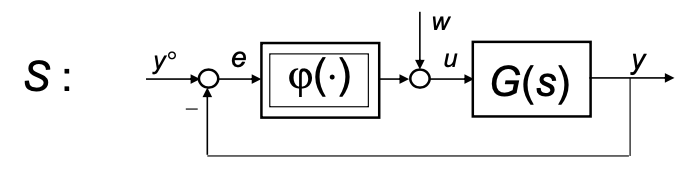
\includegraphics[scale=0.4]{immagini/l2stabsist}
	\caption{}
	\label{fig:l2stabsist}
\end{figure}
\begin{thm}[Circle criterion for $L_2$ stability of Lur'e system]
	System S is $L_2$-stable for any $\phi(\cdot)\in\Phi_{[k_1,k_2]}$ if the number of encirclements of G(s) Nyquist plot around $O(k_1,k_2)$ is equal to the number of poles of G(s) with positive real part.
	\begin{figure}[H]
		\centering
		\includegraphics[scale=0.4]{immagini/signsmatter}
		\caption{}
		\label{fig:signsmatter}
	\end{figure}
\end{thm}
IMPORTANT: here the signs matters!
\paragraph[Problem:]\newline
	Identify connections between various kinds of I/O stability and of Lyapunov stability.\\
	Results are very few.\\
	Exception: the class of linear time invariant systems.
\begin{prop}
	Given a linear time invariant dynamical system S,\begin{itemize}
		\item if S is asymptotically stable the operator H associated with S is $L_p$-stable for any $p\in(0,\infty]$
		\item If H is $L_p$-stable for any $p\in(0,\infty]$ S is asymptotically stable if and only if its non-observable and non-reachable parts are asymptotically stable.
	\end{itemize}
\end{prop}
\section{Passivity versus $L_2$ stability}
\begin{thm}[Passivity and $L_2$ stability]
	If a dynamical system S
	\begin{itemize}
		\item is strictly passive w.r.t. the output, then, the causal operator $H:\, L_{2e} \to L_{2e}$ associated with S is weakly bounded and hence $L_2$-stable, with gain smaller than or equal to $1/\delta$.
		\[
		u \, y \ge \frac{\partial V}{\partial x}(x)f(x,u)+\epsilon u^2+\delta y^2+ \rho \varphi(x),\,\forall \, (x,u)\in \Re^n \times \Re
		\]
	\end{itemize}
\end{thm}
\begin{proof}
	\[\begin{aligned}
		\dot{V}(x)&=\frac{\partial V}{\partial x}(x)f(x,u)\le u \, y -\epsilon u^2-\delta y^2 - \rho \varphi(x)\\
			&\le u \, y-\delta y^2 = -\frac{(u-\delta y)^2}{2\delta}+\frac{u^2}{2\delta}-\frac{\delta  y^2}{2}\\
			&\le \frac{u^2}{2\delta}-\frac{\delta y^2}{2}
	\end{aligned}\]
By integrating, we get 
\[
V(x(\tau))-V(x(0))\le \frac{1}{\delta^2}\int_{0}^{\tau}u^2(\tau)d\tau-\frac{\delta}{2}\int_{0}^{\tau}y^2(\tau)d\tau
\]
And, since V is positive semidefinite
\[
\|y_{\tau}\|_2^2=\int_{0}^{\tau}y^2(\tau)d\tau\,  \le\, \frac{1}{\delta^2}\int_{0}^{\tau}u^2(\tau)d\tau+\frac{2}{\delta}V(x(0))
\]
from $\sqrt{a^2+b^2}\le a+b \, (a,b>0)$ we have
\[
\|t_{\tau}\|_2\le \frac{1}{\delta}\|u_{\tau}\|_!+\sqrt{\frac{2}{\delta}V(x(0))}\qquad \forall \, (u,\tau) \in L_{2e}\times \Re^+
\]
And hence $\|y\|_2\le \gamma\|u\|_2,\quad \forall \, u \in L_2$.
\end{proof}